\chapter{Analyse}


\section{Hoe werkt het s88 protocol}
Het s88 wordt uitgelegd met behulp van onderstaande afbeelding.
\\\\
Hierin is CENTRALE is de in dit project gebruikte XILINX bord. 
\\\\
Een centrale, die hier CENTRALE heet, kan met behulp van het s88 protocol de rechter s88 bus uitlezen. Dit gebeurt met behulp van een schuifregister.
\\\\
Met de DATA OUT poort van de CENTRALE s88 BUS wordt data ingelezen. Deze is verbonden met de Q1 out poort van het schuifregister, hiermee wordt dus informatie van het schuifregister naar de CENTRALE overgedragen.
\\\\
De werking is als volgt, op het moment dat de CENTRALE een positieve flank geeft op de CLOCK en is de LATCH Hoog dan zal het schuifregister de data op Ingang D inlezen. Geeft de CENTRALE een positieve flank en is LATCH Laag dan zal de schuifregister één positie opschuiven.
\\\\
Door een puls op RESET te geven worden de buffers gereset en zijn weer gereed voor het ontvangen van nieuwe data. 


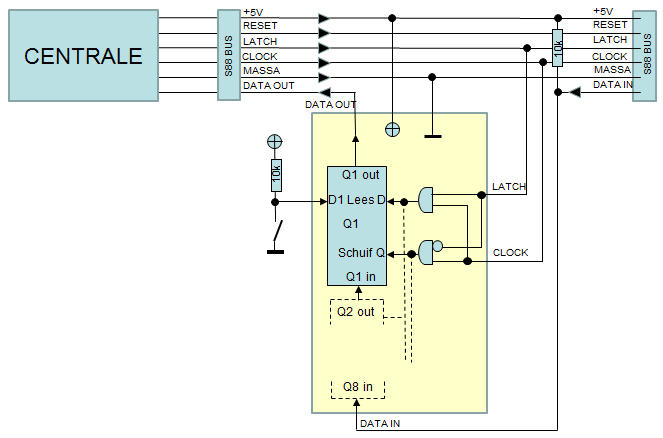
\includegraphics[width=400px]{./img/S88Bus.png}
%http://users.telenet.be/RedDeBist/MBAAN/S88%20terugmelder.htm#S88 bus:
@online{ID,
	title = {S88 TERUGMELDERS},
	date = {04-03-2016},
	url = {http://users.telenet.be/RedDeBist/MBAAN/S88%20terugmelder.htm},
		
	}
\clearpage
	
\section{Hoe werkt een XILINX Spartan 3E FPGA bord}
%http://www.xilinx.com/support/documentation/data_sheets/ds312.pdf
